%!TEX root = dippa.tex
%%% This file contains the Gene expression section of my master's thesis.
%%% This section covers the basics of gene expression.
%%% Author: Viljami Aittomäki

\section{Gene expression}\label{gene-expression}

Genetic information is encoded in deoxyribonucleic acid (DNA). A
gene is a section of DNA that serves as a template for a functional
ribonucleic acid (RNA) molecule. Gene expression refers to this process of
synthesizing a functional end-product from the information contained in gene.
DNA and gene expression serve as the basis of all currently known life. \citep{Strachan2011}

Most of gene expression is dedicated to production of proteins. The Central
Dogma of Molecular Biology, postulated by Francis Crick in 1970, describes the
general schema of how genetic information flows from genes to proteins; DNA is
first transcribed into messenger RNA (mRNA), which is then translated into
polypeptides, which ultimately form proteins \citep{Crick1970} (illustrated in
Figure \ref{fig:central-dogma}). The flow is not strictly one-directional,
though, as reverse transcriptases, a family of enzymes, can synthesize DNA
from an RNA template.

\begin{figure}[!h]
  \centering
  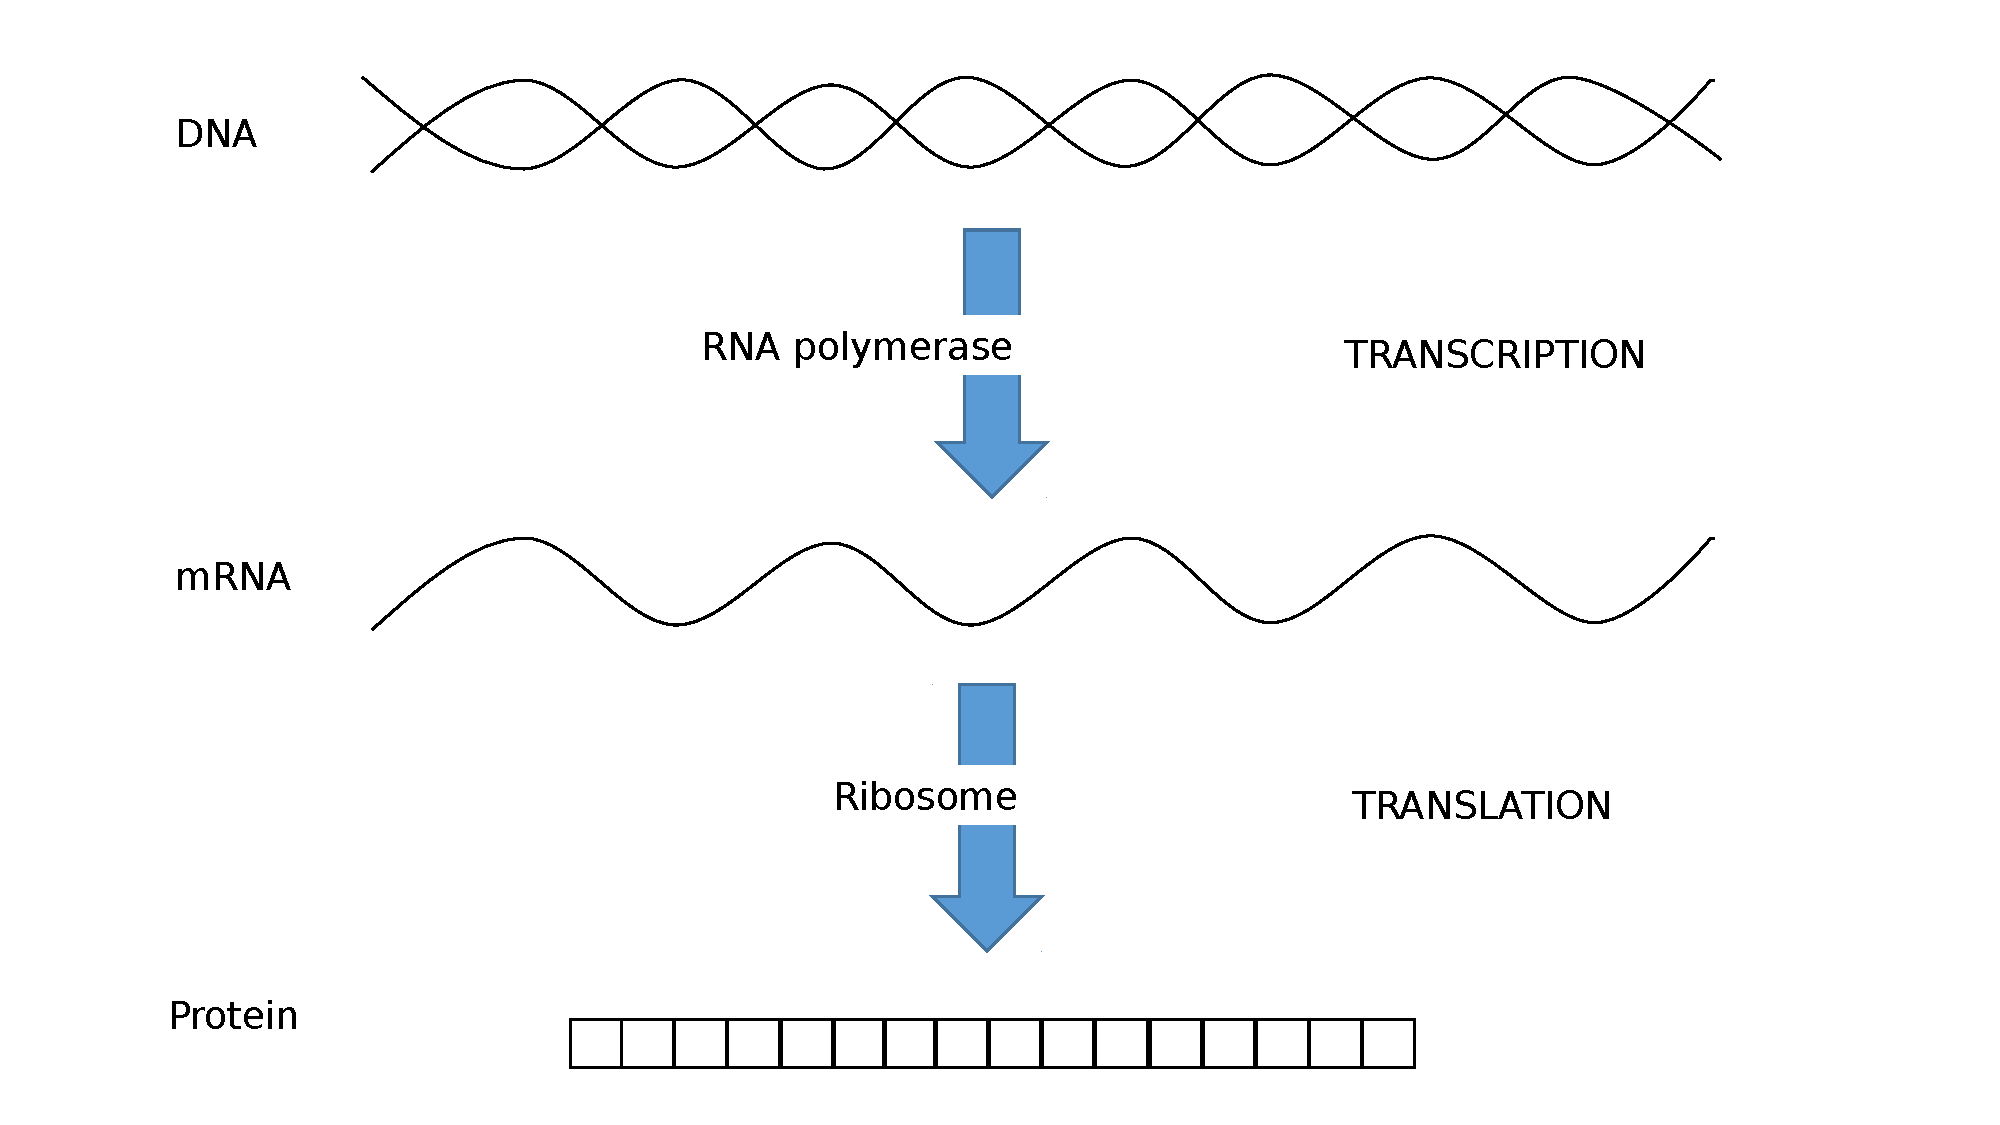
\includegraphics[width=.8\linewidth]{figures/central_dogma.pdf}
  \caption{The Central Dogma of Molecular Biology, as postulated by Crick \citep{Crick1970}.
  Most genetic information flows from DNA to RNA to protein.}
  \label{fig:central-dogma}
\end{figure}

All genes are transcribed to RNA, but all do not encode proteins. The
human genome\footnote{The genome refers to the whole genetic material of an
organism or an individual.} has been suggested to contain approximately 20 500
protein-coding genes, which encompass only around 1.5\% of the whole genetic
sequence \citep{Clamp2007}. The vast majority of the human genome was, thus,
previously thought to be without function and referred to as "junk DNA". More
recently, however, it has become evident that human DNA is pervasively
transcribed, the majority of it appears functional, and many coding and
non-coding regions overlap in the DNA \citep{Strachan2011}.

Non-coding genes give rise to non-coding RNA (ncRNA), a class of RNA molecules
that both participate in and regulate the expression of other genes.
Examples of known ncRNAs and their functions are presented in Table
\ref{table:rnas}. Nevertheless, the function and significance (if any) of many
transcribed and non-coding regions of the genome still remains unknown.

\begin{table}
  \caption{Examples of known major classes of human non-coding RNA and their
  general functions. This table is not exhaustive and several additional classes have
  been discovered. Table adapted from \citep{Strachan2011}. \\
  Size: approximate sequence lengths of each class in number of nucleotides.
  Abbrev.: abbreviations commonly used.}
  \label{table:rnas}
  \centering
  {\fontfamily{lmss}\fontsize{10pt}{12pt}\selectfont
  \begin{tabular}{ lllp{6cm} }
    \hline
    \textbf{RNA class} & \textbf{Abbrev.} & \textbf{Size (nt)} & \textbf{Function} \\
    \hline
    Ribosomal RNA         & rRNA   & 120--5000  & Components of ribosomes (which perform translation) \\
    Transfer RNA          & tRNA   & 70--80     & Transporting peptides and decoding mRNA sequence into peptides \\
    Small nuclear RNA     & snRNA  & 60--360    & Intron splicing; regulation of transcription, chromosomal replication and cell cycle etc.  \\
    MicroRNA              & miRNA  & 21--24     & Post-transcriptional gene regulation \\
    Small interfering RNA & siRNA  & 21--22     & Post-transcriptional regulation \\
    Long non-coding RNA   & lncRNA & $>$ 1000   & Gene regulation at several stages \\
    \hline
  \end{tabular}
  }
\end{table}




\subsection{Regulation of gene expression}\label{regulation-of-gene-expression}

The proper regulation of gene expression is paramount for cells to respond to
external signals, changes in their environment, and to go through different
developmental stages. Gene expression is, thus, under complex control mechanisms,
which result in tissue and cell-specific expression. This regulation
occurs on several stages including transcriptional, post-transcriptional,
translational and post-translational regulation. \citep{Strachan2011}

The first step of this regulation is control of transcription. To be
transcribed, genes need active initiation of transcription, which
occurs in the promotor regions. While the actual transcription is performed by
RNA polymerases, many different transcription factors and regulatory proteins
participate in its regulation. Transcription is possible only when
the chromatin structure of the transcribed genetic region is opened from its
tight package around histone proteins, which is controlled by additional
factors such as histone acetylation.

The produced mRNA undergoes post-transcriptional modifications, such as
capping, polyadenylation and splicing of introns, which all are essential for
further translation of the mRNA to protein \citep{Strachan2011}. All these
steps must maintain a certain level of fidelity, as even slight structural
changes can render both mRNA and protein to degradation and. The main
post-transcriptional control mechanism seems to be RNA interference (RNAi). It
causes suppression of gene expression through mRNA degradation and inhibition of translation.
MicroRNAs (miRNAs) and small interfering RNAs (siRNAs) are central components of the
RNAi pathway; they act as target mRNA recognizing templates.
While miRNAs are cut from endogenous hairpin structures, siRNAs, however,
are mostly processed from exogenous long double-stranded RNAs
(dsRNAs)\footnote{The mechanism of RNAi has been postulated to having evolved
as a defense mechanism against dsRNA coming from pathogens.} \cite{Du2005}. MicroRNAs,
which are the focus of this study, are discussed in more detail in the next section.

The translation of mRNA to protein can also be directly regulated, but this
seems less prevalent than control of previous phases. Post-translationally,
proteins can be modified and degraded to affect their function and cellular
expression levels \citep{Strachan2011}.




\subsection{Measuring gene expression}\label{measurement-of-gene-expression}

The physical measurement of gene expression can be done on either the level of
messenger RNA molecules or protein molecules. Although proteins are the
eventual effector molecules -- at least for protein-coding genes
-- gene expression is usually thought to be synonymous with mRNA expression.
mRNA abundances are significantly easier to measure
than protein abundances, due to the chemistry of hybridization and
the relative ease of replicating DNA and RNA sequences by exploiting cellular
machinery evolved for this purpose.

Quantitative PCR (qPCR) is a DNA/RNA measurement method based on the
polymerase chain reaction (PCR) that provides a quantitative measurement of
PCR products. qPCR is considered a golden standard in gene expression
measurement and is widely used in research, but also in clinical diagnostics.
It is often the method of choice for measuring a moderate number of genes. \citep{VanGuilder2008}

Gene expression microarrays are based on probes printed on a
surface, where each probe is designed to hybridize with a specific mRNA.
The advantage of microarrays is that they allow massively
parallel analysis of even whole genomes simultaneously. They are also relatively inexpensive and
easy to use, making them a ubiquitous tool for expression measurements. Detection
of expression levels is based on fluorescence and optical sensors, and
therefore subject to noise. As microarray data are inherently noisy, proper
normalization methods have been shown to be important. Probe designs can also
become obsolete as reference genomes are updated and, therefore, reassessment
of the true targets of probes is advisable. \citep{Allison2006}

More recently next generation sequencing methods have been applied to gene
expression profiling. These are not dependent on previous reference sequences,
but are relatively expensive and laborious compared to microarrays.

Protein expression can be measured using several different methods. Perhaps most widely
used are different variations of mass spectrometry (MS). Application of MS methods is
limited by their resource-intensiveness and poor scaling, however. Reverse phase protein
arrays (RPPA) are a platform similar to microarrays, where protein samples are fixated
to a solid surface and then probed with antibodies binding to a specific proteins.
RPPAs are inexpensive, allow large-scale analyses, and analysis of RPPA data is
similar to microarrays, making them an attractive choice for studies
using multiomics data \citep{Mannsperger2010}.

The general assumption has been that mRNA expression is representative of gene
expression and that changes in mRNA abundances also reflect changes in protein
abundances. This assumption has recently been challenged by experiments
indicating that correlations between the expression of mRNA and corresponding
protein are low, with mRNA expression explaining around 40\% of variation in
protein expression \citep{Vogel2012}.
Payne recently concluded that "proteome and transcriptome
abundances are not sufficiently correlated to act as proxies for each other"
and that most of this difference is likely caused by biological regulation and
not by measurement technology \cite{Payne2015}.
% This regulation can be post-transcriptional, translational
% or protein-degradation related, as discussed above.
Therefore, it is interesting, even necessary, to integrate measurements from
different stages of gene expression -- for example mRNA, microRNA and protein
abundances -- to gain new insights into biological processes.


% Some studies have reported
% modest to good correlation, however, and one study suggested that mRNA-protein
% correlations are generally higher for genes that have differing mRNA
% expression between studied conditions (e.g. cancerous versus healthy tissue)
% \citep{Koussounadis2015}, indicating that, while correlation is perhaps low in
% general, changes in mRNA expression cause detectable changes in protein
% expression.

